% \begin{minipage}[b]{0.6\linewidth}
\begin{center}
  \resizebox{13cm}{!}{%
    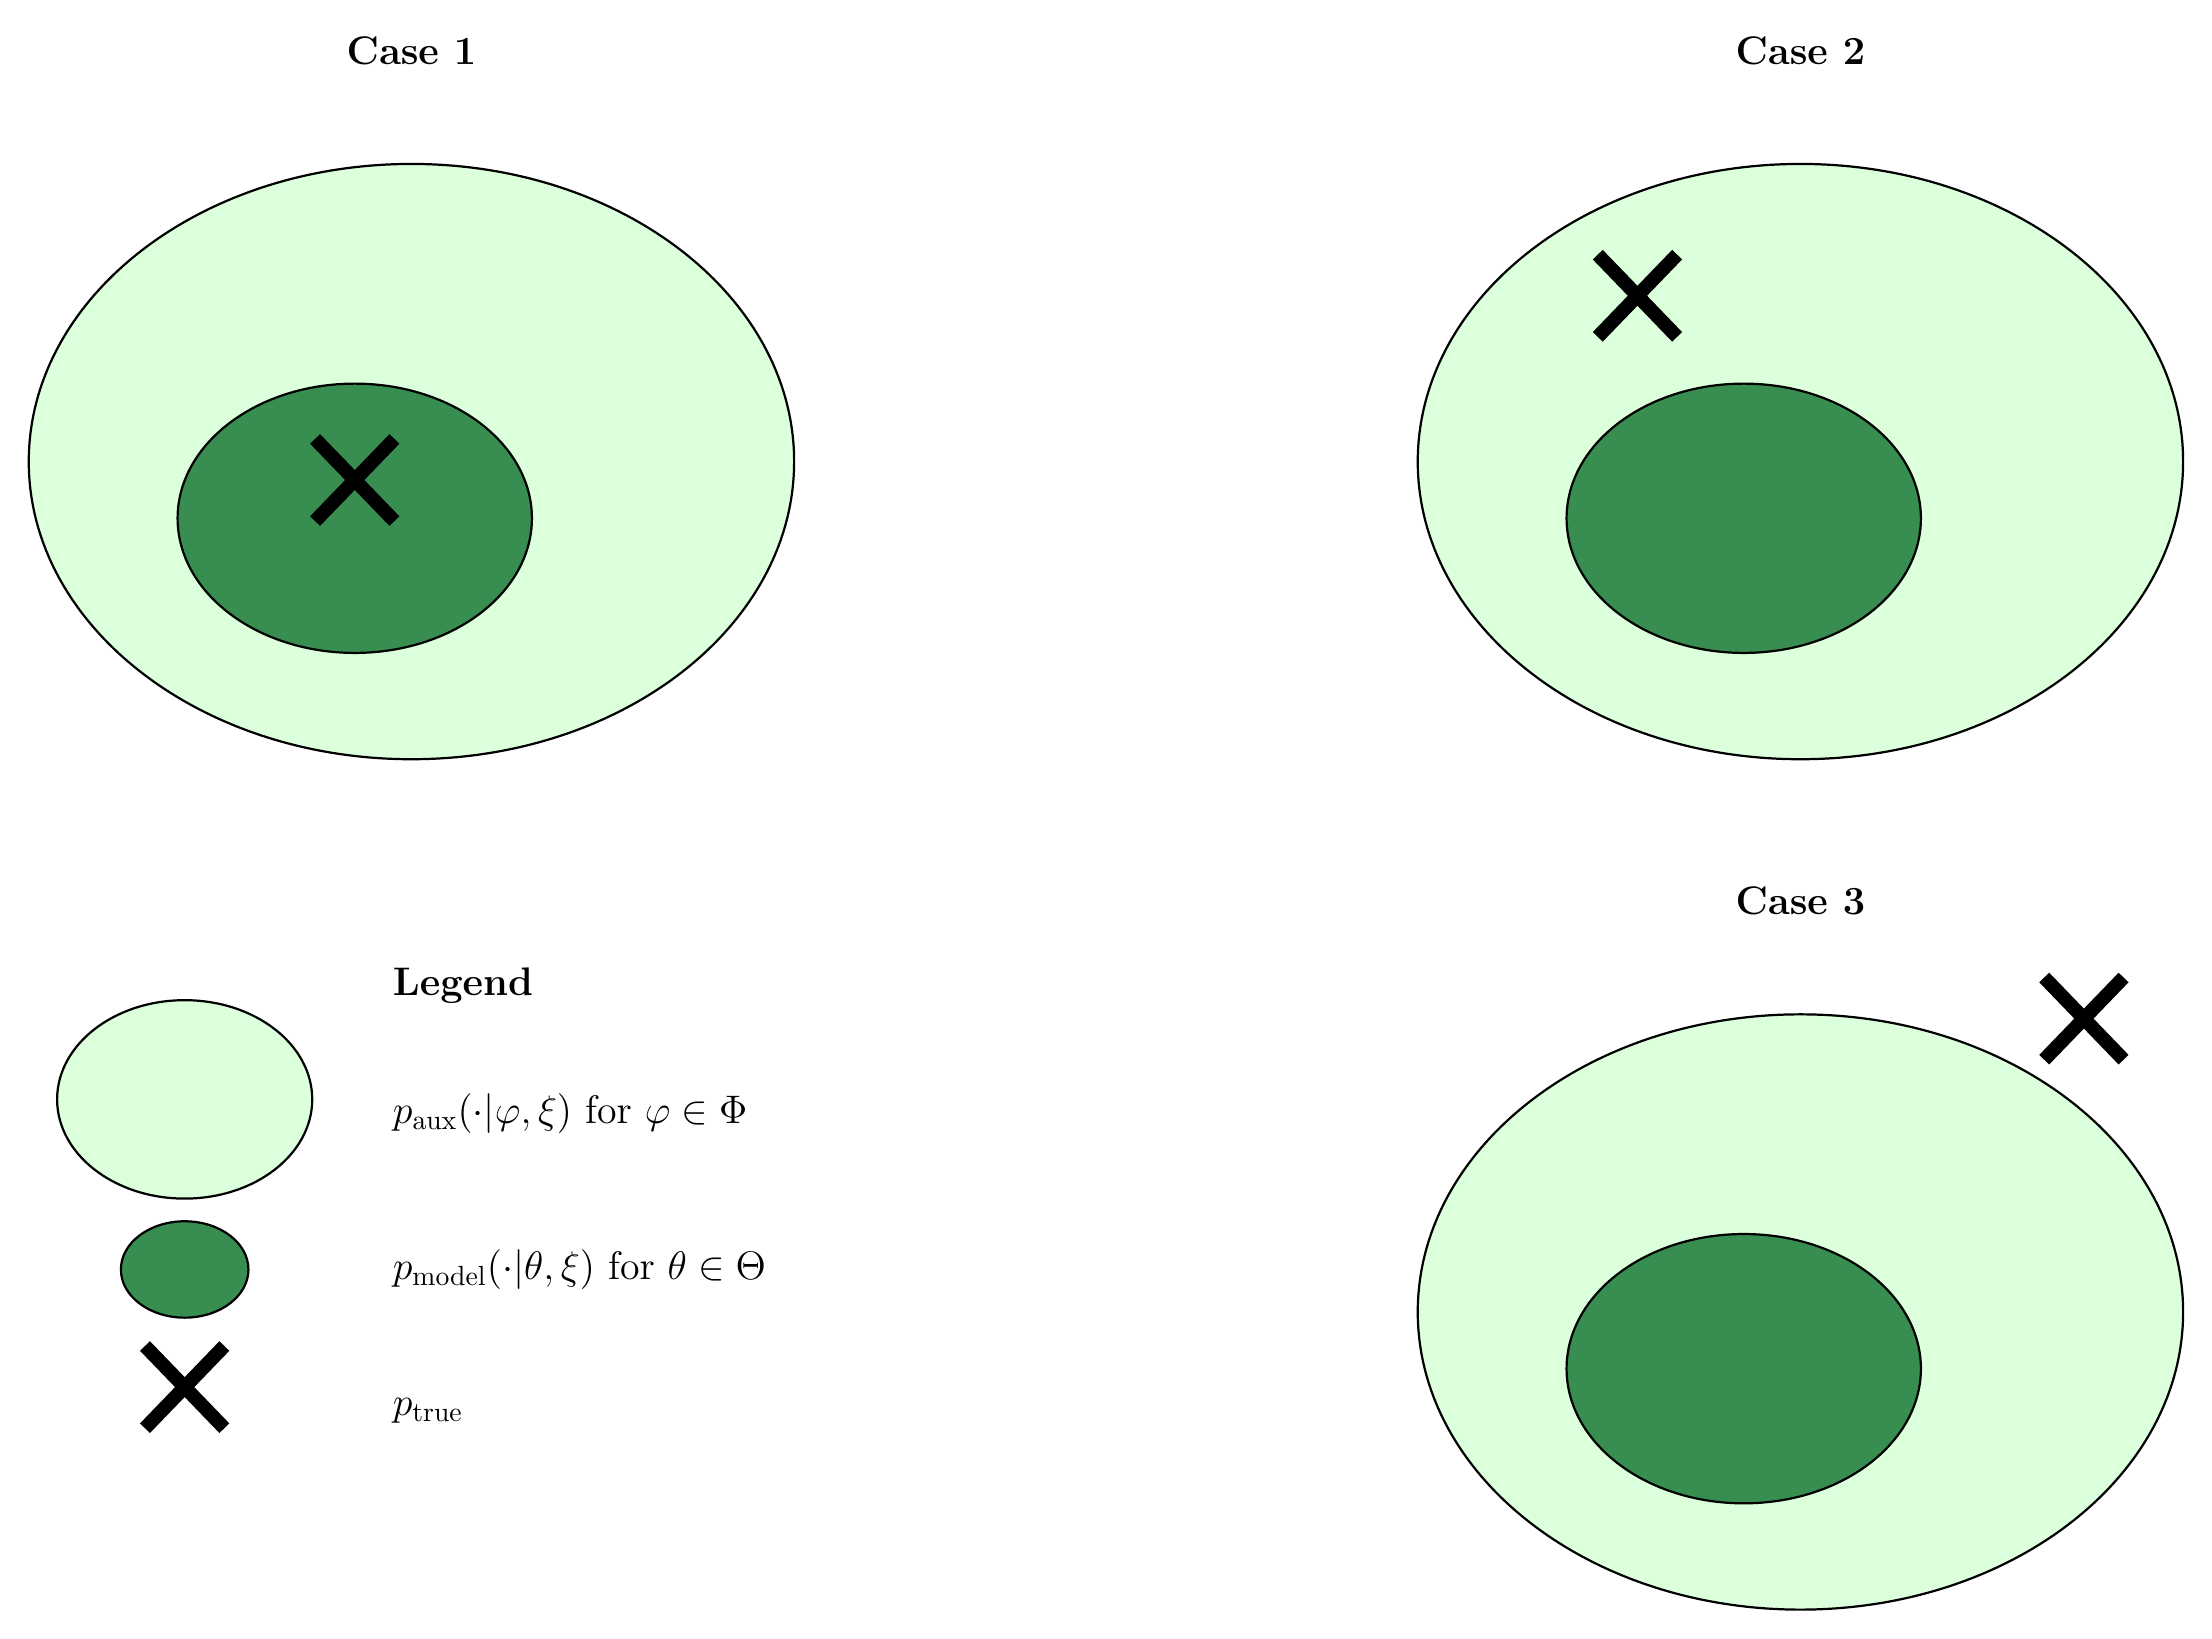
\begin{tikzpicture}[font=\sffamily, >=stealth]

      % Colors: light and dark green
      %\definecolor{auxfill}{RGB}{212,237,218}   % light green
      \definecolor{auxfill}{RGB}{220,255,220}

      \definecolor{modelfill}{RGB}{56,142,80}   % darker green

      % scale factor to make whole thing slightly bigger
      \def\myscale{1.8}

      % --- Top-left panel: Case 1 ---
      \begin{scope}[scale=\myscale, shift={(-5.0,3.2)}]
        % header
        \node[font=\bfseries\Large] at (0,2.9) {Case 1};

        % outer ellipse: p_aux (phi)
        \fill[auxfill] (0,0) ellipse (2.7cm and 2.1cm);
        \draw[thick] (0,0) ellipse (2.7cm and 2.1cm);

        % inner ellipse: p_model (theta)
        \fill[modelfill] (-0.4,-0.4) ellipse (1.25cm and 0.95cm);
        \draw[thick] (-0.4,-0.4) ellipse (1.25cm and 0.95cm);

        % % inner labels
        % \node[below=18pt, font=\Large] at (0,0) {$p_{\mathrm{model}}(\cdot;\theta)$};
        % \node[below=36pt, font=\Large] at (0,0) {$p_{\mathrm{aux}}(\cdot;\phi)$};

        % % p_true marker inside p_model (large X) and label
            \begin{scope}[shift={(-0.4,-0.4)}]
          \draw[line width=5pt] (-0.28,-0.02) -- (0.28,0.56);
          \draw[line width=5pt] (-0.28,0.56) -- (0.28,-0.02);
        \end{scope}
        % \node[right=6pt, font=\Large] at (0.75,0.25) {$p_{\mathrm{true}}$};
      \end{scope}

      % --- Top-right panel: Case 2 ---
      \begin{scope}[scale=\myscale, shift={(4.8,3.2)}]
        % header
        \node[font=\bfseries\Large] at (0,2.9) {Case 2};

        % outer ellipse: p_aux (phi)
        \fill[auxfill] (0,0) ellipse (2.7cm and 2.1cm);
        \draw[thick] (0,0) ellipse (2.7cm and 2.1cm);

        % inner ellipse: p_model (theta)
        \fill[modelfill] (-0.4,-0.4) ellipse (1.25cm and 0.95cm);
        \draw[thick] (-0.4,-0.4) ellipse (1.25cm and 0.95cm);

        % inner labels
        % \node[below=18pt, font=\Large] at (0,0) {$p_{\mathrm{model}}(\cdot;\theta)$};
        % \node[below=36pt, font=\Large] at (0,0) {$p_{\mathrm{aux}}(\cdot;\phi)$};

        % % p_true marker inside p_aux but outside p_model (large X) and label
            \begin{scope}[shift={(-1.15,0.9)}]
          \draw[line width=5pt] (-0.28,-0.02) -- (0.28,0.56);
          \draw[line width=5pt] (-0.28,0.56) -- (0.28,-0.02);
        \end{scope}
        % \node[font=\Large] at (-0.3,1.55) {$p_{\mathrm{true}}$};
      \end{scope}

      % --- Bottom-right panel: Case 3 ---
      \begin{scope}[scale=\myscale, shift={(4.8,-2.8)}]
        % header
        \node[font=\bfseries\Large] at (0,2.9) {Case 3};

        % outer ellipse: p_aux (phi)
        \fill[auxfill] (0,0) ellipse (2.7cm and 2.1cm);
        \draw[thick] (0,0) ellipse (2.7cm and 2.1cm);

        % inner ellipse: p_model (theta)
        \fill[modelfill] (-0.4,-0.4) ellipse (1.25cm and 0.95cm);
        \draw[thick] (-0.4,-0.4) ellipse (1.25cm and 0.95cm);

        % inner labels
        % \node[below=18pt, font=\Large] at (0,0) {$p_{\mathrm{model}}(\cdot;\theta)$};
        % \node[below=36pt, font=\Large] at (0,0) {$p_{\mathrm{aux}}(\cdot;\phi)$};

        % % p_true marker outside both (large X) and label
         \begin{scope}[shift={(2.0,1.8)}]
           \draw[line width=5pt] (-0.28,-0.02) -- (0.28,0.56);
           \draw[line width=5pt] (-0.28,0.56) -- (0.28,-0.02);
         \end{scope}
        % \node[right=6pt, font=\Large] at (1.95,1.6) {$p_{\mathrm{true}}$};
      \end{scope}

      % --- Bottom-left legend / key ---
      \begin{scope}[scale=\myscale, shift={(-5.0,-2.0)}]
        \node[font=\bfseries\Large, anchor=west] at (-0.2,1.5) {Legend};

        % key: aux (large ellipse)
        \fill[auxfill] (-1.6,0.7) ellipse (0.9cm and 0.7cm);
        \draw[thick] (-1.6,0.7) ellipse (0.9cm and 0.7cm);
        \node[anchor=west,font=\Large] at (-0.2,0.6) {$p_{\mathrm{aux}}(\cdot|\varphi,\xi)$ for $\varphi \in \Phi$};

        % key: model (small ellipse)
        \fill[modelfill] (-1.6,-0.5) ellipse (0.45cm and 0.34cm);
        \draw[thick] (-1.6,-0.5) ellipse (0.45cm and 0.34cm);
        \node[anchor=west,font=\Large] at (-0.2,-0.5) {$p_{\mathrm{model}}(\cdot|\theta,\xi)$ for $\theta \in \Theta$};

        % key: p_true (large X)
        \begin{scope}[shift={(-1.6,-1.6)}]
          \draw[line width=5pt] (-0.28,-0.02) -- (0.28,0.56);
          \draw[line width=5pt] (-0.28,0.56) -- (0.28,-0.02);
        \end{scope}
        \node[anchor=west,font=\Large] at (-0.2,-1.5) {$p_{\mathrm{true}}$};

      \end{scope}

    \end{tikzpicture}
  } % end resizebox

\end{center}
% \end{minipage}%
% \begin{minipage}[b]{0.4\linewidth}
%     \vspace{0.5cm}


% \end{minipage}
% \begin{figure}[ht!]
%   \caption{Three cases for the true data-generating distribution $p_{\mathrm{true}}$ relative to the model family $p_{\mathrm{model}}(\cdot;\theta)$ and the auxiliary set $p_{\mathrm{aux}}(\cdot;\phi)$.}
%   \label{fig:pt_true_cases}
% \end{figure}

% \begin{itemize}
%     \item \textbf{Case 1:} In this case we have that there exist parameter values $\theta$ such that our model matches the true data generating process. It is not misspecified.
%     \item \textbf{Case 2:} In this case there do not exist parameter values $\theta$ such that our model matches the true data generating process. However, there are some parameters such that our auxiliary model class fit the true data generating process. In this case the model is misspecified.
%     \item \textbf{Case 3:} Again the model is misspecified. However, in this case the true data generating process in neither in our model class, nor our auxiliary model class.
% \end{itemize}


% We have our extended model, $p_{\mathrm{ext}}$, given by,

% \[\begin{aligned}
% \theta &\sim p_{\theta}(\cdot), \qquad
% \psi \sim p_{\psi}(\cdot), \qquad
% Z \sim \mathrm{Bernoulli}(1-\varepsilon),\\[4pt]
% \forall t=1,\dots,T\quad &\xi_t = \pi_t(h_{t-1}),\\[4pt]
% y_t &\sim
% \begin{cases}
% p_{\mathrm{model}}(\,\cdot\mid \theta,\xi_t) & \text{if } Z=1,\\[4pt]
% p_{\mathrm{aux}}(\,\cdot\mid \psi,\xi_t)   & \text{if } Z=0.
% \end{cases}
% \end{aligned}
% \]




% We have the expected divergence ($\mathrm{ED}$) between our assumed model and the true model, given a past history of experiments, $h_t$, 

% \[
% \mathrm{ED}(h_t)
% = \mathbb{E}_{p(x^*)}\!\left[ 
%     \mathrm{KL}\!\left( p_{\mathrm{true}}(y^* \mid x^*) \,\big\|\, 
%                         p_{\mathrm{model}}(y^* \mid x^*, h_t) \right)
% \right].
% \]

% Instead we could phrase this as, 

% \[
% \mathrm{ED}(h_t)
% = \mathbb{E}_{p(x^*)}\!\left[
%     D_{\varphi}\!\big( p_{\mathrm{true}}(\cdot\mid x^*) \,\big\|\, p_{\mathrm{model}}(\cdot\mid x^*,h_t) \big)
% \right],
% \]

% and so now 



% -------------------------------------------------------
% DEFINITIONS
% -------------------------------------------------------

% \begin{definition}[Design and Observations]
% Let $\xi_t \in \mathcal{X}$ denote the design chosen at iteration $t$ and 
% $y_t \in \mathcal{Y}$ the corresponding experimental outcome.  
% The sequence of collected data up to time $t$ is
% \[
% h_t := \{(\xi_i, y_i)\}_{i=1}^t .
% \]
% A design policy $\pi_t$ maps histories to designs, i.e.
% \[
% \xi_t = \pi_t(h_{t-1}).
% \]
% \end{definition}